Firebase es una plataforma propiedad de Google que tiene como objetivo proporcionar un enfoque completo para un rápido desarrollo web y móvil. En resumen, le permite centrarse en las partes frontales de la aplicación. Se completa con una base de datos NoSQL, alojamiento, almacenamiento de archivos, procesamiento del lado del servidor para cosas que deben protegerse de la interfaz y un sistema de autenticación, que junto a módulos de desarrollo \textit{frontend} como ReactJS, proporcionan todo lo necesario para crear aplicaciones web pequeñas y medianas.
\vspace{0.8cm}

\subsection{Componentes FERN}
\begin{itemize}
  \item Firebase (base de datos)
  \item Express.js (servidor)
  \item ReactJS (cliente)
  \item Node.js (entorno del servidor)
\end{itemize}
\begin{figure}[H]
  \centering
  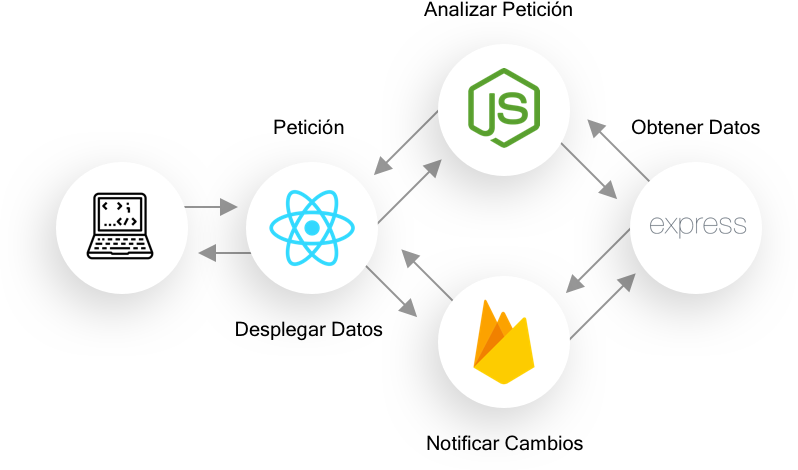
\includegraphics[width=0.8\textwidth]{fern}
  \caption{Flujo de información en FERN Stack.}
\end{figure}

\subsection{Cloud Firestore}
Firestore es una bases de datos orientada a documentos, toda la información se guarda en colecciones como JSON, principalmente diseñada para almacenar, recuperar y administrar información orientada a documentos, también conocida como datos semiestructurados.
\vspace{0.8cm}

La escalabilidad es completamente automática, lo que significa que no es necesario compartir sus datos en varias instancias. Los cargos de Cloud Firestore se basan en las operaciones realizadas en su base de datos (lectura, escritura, borrado), ancho de banda y almacenamiento. Admite límites de gasto diario para proyectos de Google App Engine, para garantizar que no exceda los costos con los que el usuario se sienta cómodo.
\begin{figure}[H]
  \centering
  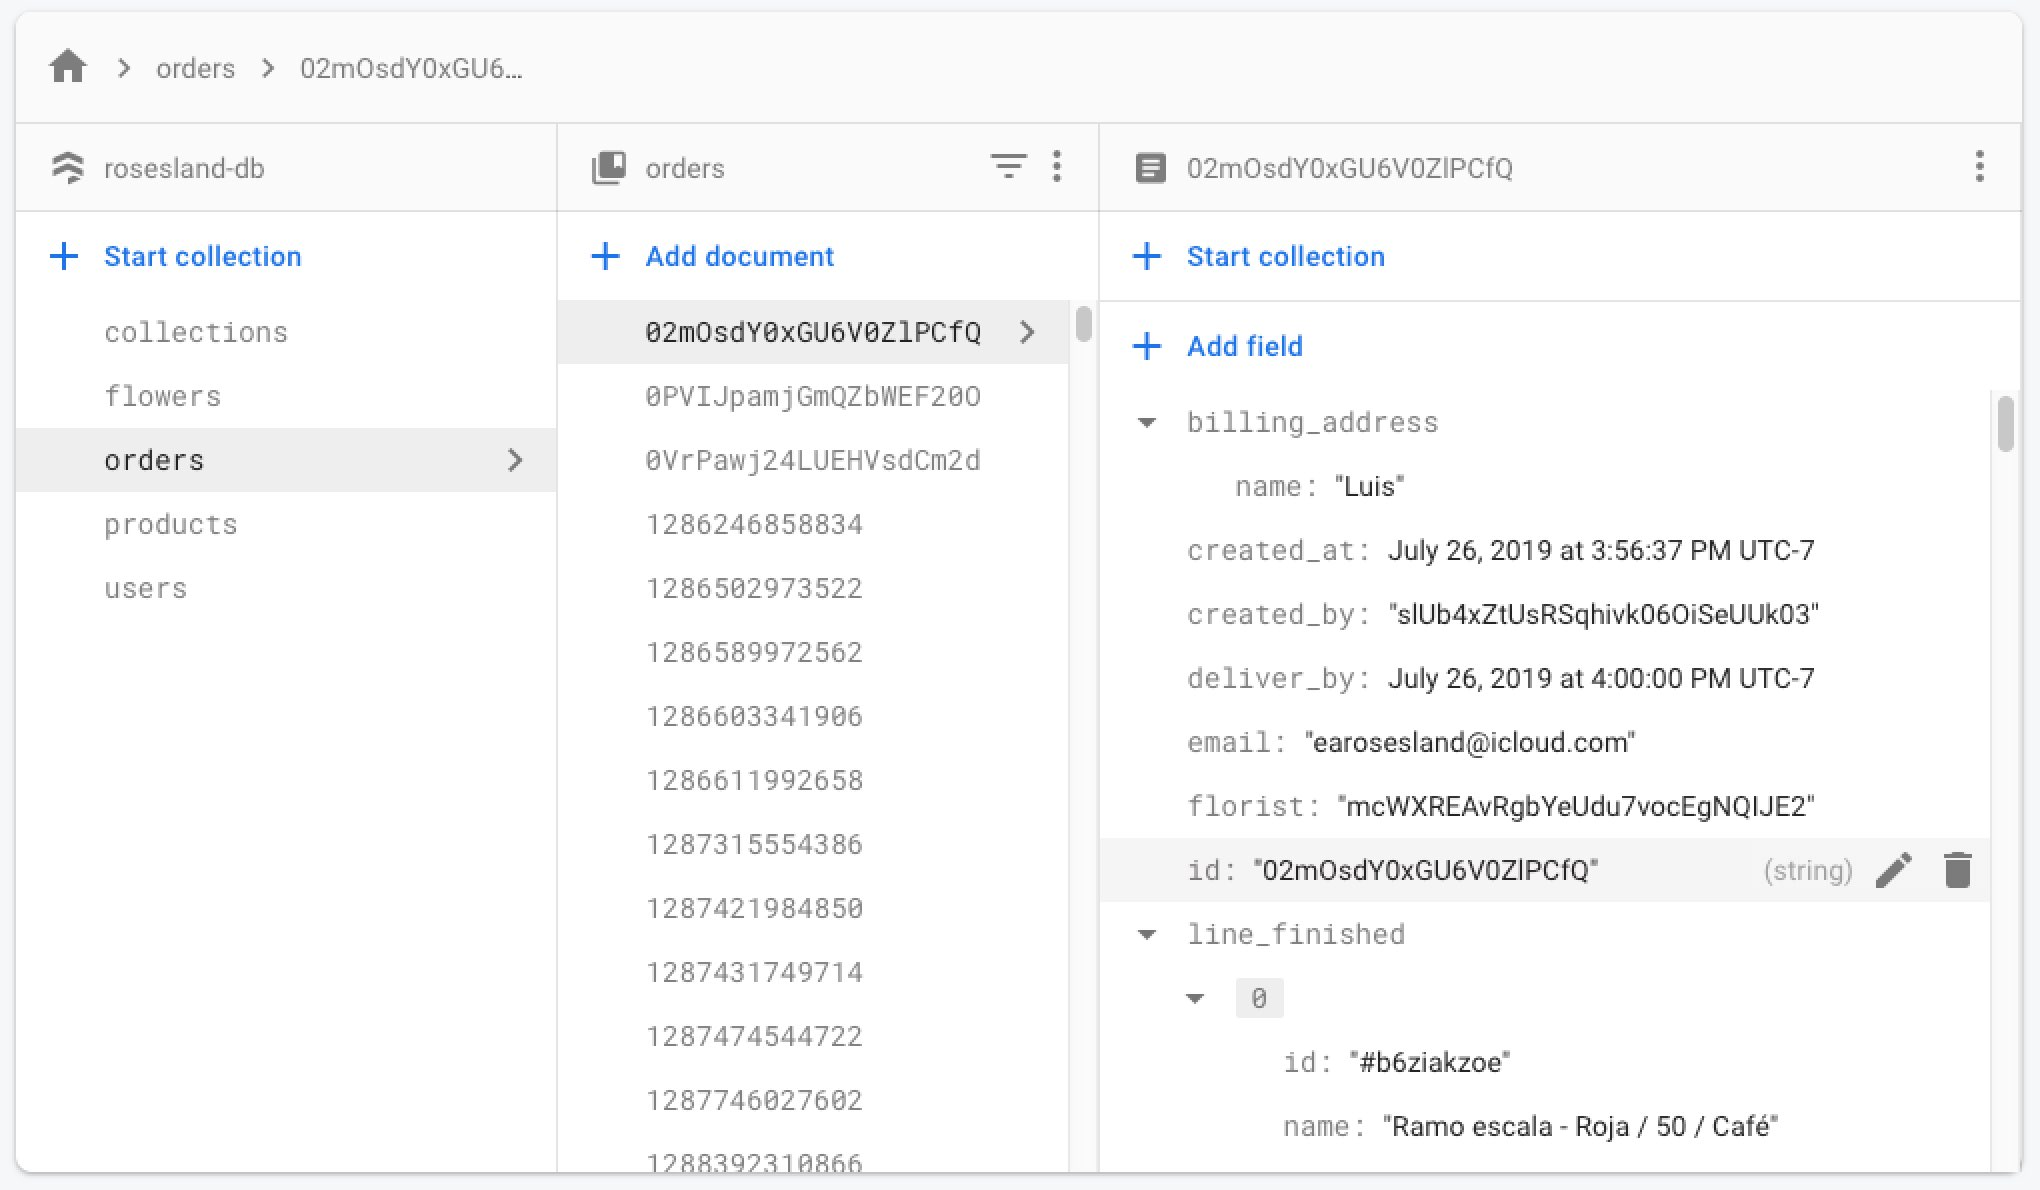
\includegraphics[width=0.9\textwidth]{firestore}
  \caption{Colección de Firestore con sus documentos internos.}
\end{figure}

\subsection{Node.js}
Node.js es un entorno multiplataforma de código abierto para ejecutar código JavaScript del lado del servidor. El entorno de tiempo de ejecución de Node.js incluye todo lo que necesita para ejecutar un programa escrito en JavaScript. 
\vspace{0.8cm}

Node.js surgió cuando los desarrolladores originales de JavaScript lo extendieron de algo que solo podía ejecutar en el navegador a algo que podría ejecutar en su máquina como una aplicación independiente. Ahora puede hacer mucho más con JavaScript que simplemente hacer que los sitios web sean interactivos. JavaScript ahora tiene la capacidad de hacer cosas que otros lenguajes de secuencias de comandos como Python pueden hacer. Tanto su navegador JavaScript como Node.js se ejecutan en el motor de tiempo de ejecución JavaScript V8. Este motor toma su código JavaScript y lo convierte en un código de máquina más rápido. El código de máquina es un código de bajo nivel que la computadora puede ejecutar sin necesidad de interpretarlo primero.
\vspace{0.8cm}

\begin{figure}[H]
  \centering
  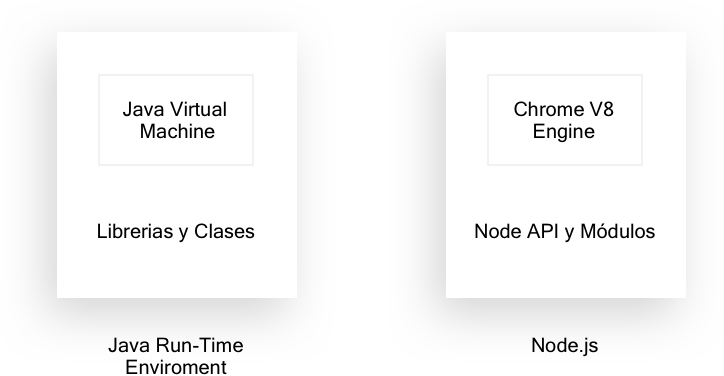
\includegraphics[width=0.8\textwidth]{node}
  \caption{Analogía Node.js con Java.}
\end{figure}
% \vspace{0.8cm}

\subsubsection{Motor V8 de Google Chrome}
Node.js utiliza el motor de ejecución ultra rápido V8 de Google Chrome. Hasta el lanzamiento de Chrome, la mayoría de los navegadores leían JavaScript de manera ineficiente: el código se leía e interpretaba poco a poco. Tomó mucho tiempo leer JavaScript y convertirlo a lenguaje máquina para que el procesador pudiera entenderlo. 
\vspace{0.8cm}

El motor V8 de Google Chrome funciona completamente diferente. Está altamente optimizado y lleva a cabo lo que llamamos compilación JIT (Just In Time). Transforma rápidamente el código JavaScript en lenguaje máquina.
\vspace{0.8cm}

\begin{table}[H]
  \renewcommand{\arraystretch}{1.5}
  \centering
  \scriptsize
  \begin{tabular}{ |p{2cm}||p{5cm}|p{5cm}|  }
    \hline
        Navegador
      & Motor de renderizado / diseño
      & Motor de secuencias de comandos \\
    \hline
        Chrome
      & Blink (C++)
      & V8 (C++) \\
    \hline
    \hline
        Mozilla Firefox
      & Gecko (C++)
      & SpiderMonkey (C/C++) \\
    \hline
    \hline
        IE Edge
      & EdgeHTML (C++)
      & Chakra JavaScript engine (C++) \\
    \hline
    \hline
    Opera
      & Blink (C++)
      & V8 (C++) \\
    \hline
    Internet Explorer
      & Trident (C++)
      & Chakra JScript engine (C++) \\
    \hline
  \end{tabular}
  \caption{Motores de renderizado y secuencias de comandos}
\end{table}
\vspace{0.8cm}


\subsection{El ecosistema NPM}
NPM (Node Package Manager) es el administrador de paquetes predeterminado para Node.js. Paquete es un término utilizado por npm para denotar herramientas que los desarrolladores pueden usar para sus proyectos \cite{goalkicker-node}. Se instala en el sistema con la instalación de Node.js. Los paquetes y módulos necesarios en un proyecto Node se instalan utilizando \textit{npm}.
\vspace{0.8cm}

NPM consta de tres componentes:
\begin{enumerate}
  \item Sitio web
  \item Registro
  \item CLI
\end{enumerate}
\subsubsection{Sitio web}
El sitio web oficial de npm es https://www.npmjs.com/. Con este sitio web puede encontrar paquetes, ver documentación, compartir y publicar paquetes.
\subsubsection{Registro}
El registro npm es una gran base de datos que consta de más de medio millón de paquetes. Los desarrolladores descargan paquetes del registro npm y publican sus paquetes en el registro.
\subsubsection{CLI (interfaz de línea de comando)}
Esta es la línea de comando que ayuda a interactuar con el npm para instalar, actualizar y desinstalar paquetes y administrar dependencias.
\subsection{Comandos NPM}
Npm tiene muchos paquetes que puedes usar en una aplicación para que su desarrollo sea más rápido y eficiente. Instalar módulos usando NPM no representa un gran problema. Hay una sintaxis simple para instalar cualquier módulo Node.js:
\vspace{0.8cm}

% \begin{verbatim}
%   npm install nombre-del-paquete
%   ejemplo: npm install express
% \end{verbatim}
\begin{lstlisting}[language=HTML]
  npm install nombre-del-paquete
  ejemplo: npm install express
\end{lstlisting}
% \lstinputlisting[style=ES6, caption=Comandos para instalar paquete con NPM]{code/npm.txt}

\subsection{Express.js}
Escribir un servidor web completo a mano en Node.js directamente no es tan fácil, ni es necesario, Express.js es un paquete de aplicación web minimalista y extensible creado para el ecosistema Node.js. Permite crear un servidor web legible, flexible y fácil de mantener.
\vspace{0.8cm}

Express.js le permite definir rutas, especificaciones de qué hacer cuando llega una solicitud HTTP que coincide con un patrón determinado. La especificación coincidente se basa en expresiones regulares (regex) y es muy flexible, como la mayoría de los otros entornos de aplicaciones web. La parte de qué hacer es solo una función que recibe la solicitud HTTP analizada.
\vspace{0.8cm}

Express.js analiza la URL de solicitud, encabezados y parámetros. En el lado de la respuesta, tiene, como se esperaba, toda la funcionalidad requerida por las aplicaciones web. Esto incluye la configuración de códigos de respuesta, configuración de \glspl{cookie}, envío de encabezados personalizados, etc. Además, puede escribir middleware Express, piezas de código personalizadas que se pueden insertar en cualquier ruta de procesamiento de solicitud/respuesta para lograr una funcionalidad común como el registro, la autenticación, entre otras.
\vspace{0.8cm}


\lstinputlisting[style=ES6, caption=Simple aplicación Express.js]{code/express.js}

\subsection{ReactJS}
React es una biblioteca de JavaScript declarativa, eficiente y flexible creada en 2013 por el equipo de desarrollo de Facebook. React quería que las interfaces de usuario fueran más modulares (o reutilizables) y más fáciles de mantener. Según el sitio web de React, se utiliza para \textit{construir componentes encapsulados que administran su propio estado, y unirlos para crear interfaces de usuario complejas}. React es una biblioteca JavaScript que permite componer interfaces de usuario complejas a partir de piezas de código pequeñas y aisladas llamadas \textit{componentes}.
\vspace{0.8cm}

En términos generales, al crear aplicaciones con ReactJS, se crean componentes que corresponden a distintos elementos de una interfaz de usuario. Después se organizan estos elementos dentro de componentes de orden superior que definen la estructura de la aplicación. Es importante destacar que cada componente en una aplicación React se rige por principios estrictos de gestión de datos. Interfaces avanzadas comúnmente involucran datos complejos y manejo de estado. ReactJS es limitado y tiene como objetivo darnos las herramientas para poder anticipar cómo se verá una aplicación con un conjunto de circunstancias dado.

\subsection{Componentes React}
Un componente es una pequeña parte de la interfaz de usuario. Todas las piezas reutilizables de una página web se abstraen en estos elementos. Son similares, en conceptos, a cosas como \glspl{widget} y módulos. React se define a sí mismo como una biblioteca para construir interfaces de usuario. Como tal, cuando se piensa en una interfaz de usuario, se debe pensar en ella en términos de los componentes más pequeños posibles que se puedan definir. La razón por la que existe este paradigma es para disminuir el acoplamiento (cuánto dependen los unos de los otros) y aumentar la cohesión (qué tan bien funcionan juntas las diferentes cosas).
\vspace{0.8cm}

Cada uno de estos fragmentos es un bloque de código independiente y reutilizable, que divide la interfaz de usuario en partes más pequeñas. Incluyen código que define cómo se crean los elementos en el \acrshort{dom} y cómo los usuarios pueden interactuar con ellos. Los componentes se pueden definir únicamente en JavaScript o se pueden definir en un superconjunto (o variación extendida) de JavaScript llamado JSX, que se explica en temas posteriores.
\vspace{0.8cm}

\begin{figure}[H]
  \centering
  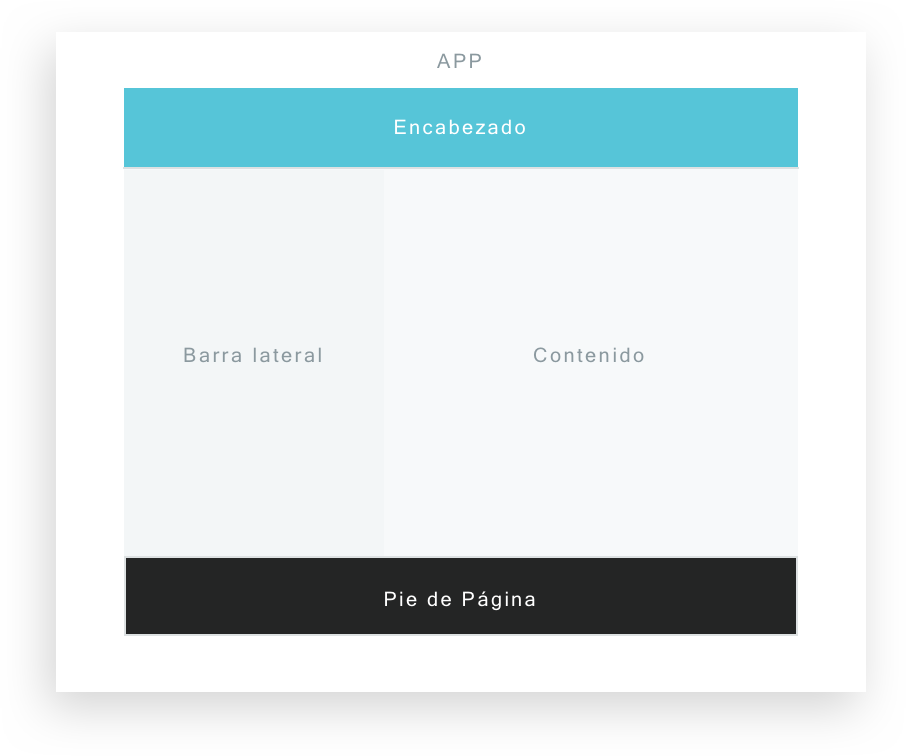
\includegraphics[width=0.8\textwidth]{components}
  \caption{Componentes principales de una página web. (Fuente: Elaboración propia)}
\end{figure}
En primer lugar, hay un elemento principal llamado componente APP. Este componente de la aplicación contiene cuatro fragmentos secundarios o se divide en cuatro componentes:
\begin{enumerate}
  \item Encabezado
  \item Barra lateral
  \item Contenido
  \item Pie de página
\end{enumerate}
La función de cada componente se manejará independientemente con otros componentes. Cada componente es una pieza reutilizable, y se puede pensar en cada componente de forma aislada.
\vspace{0.8cm}

Dentro de un componente, tendremos subcomponentes o componentes dentro de un componente padre. Esos serán reutilizables también. En pocas palabras, un componente es una clase o función de JavaScript que opcionalmente acepta entradas, es decir, propiedades (props) y devuelve un elemento que describe cómo debería lucir una sección de la interfaz de usuario.
\vspace{0.8cm}

\lstinputlisting[style=ES6, caption=Ejemplo de página con componentes ReactJS]{code/react-example.js}

\subsection{DOM Virtual}
En el desarrollo web de software, \acrshort{dom} significa Modelo de Objeto de Documento (Document Object Model) y representa la estructura de los elementos en una página web. El HTML DOM se construye como un árbol de objetos.

Algunas bibliotecas de JavaScript, como jQuery, manipulan los elementos DOM directamente, cambiando sus atributos, agregando o eliminando componentes. Sin embargo, en lugar de cambiar el DOM directamente, React usa un DOM virtual, que es una replicación virtual del árbol DOM actual. En consecuencia, React puede manipular el DOM virtual innumerables veces y comparar su estado con el DOM real. De esta manera, React sabe exactamente qué elemento cambió y luego actualiza solo ese elemento específico en la pantalla.

Detrás de escena, React hace un gran trabajo para editar y volver a \gls{renderizar} eficientemente el DOM cuando algo en la interfaz necesita cambiar. Este enfoque le brinda al desarrollador una gran flexibilidad y sorprendentes ganancias de rendimiento porque ReactJS calcula con anticipación qué cambios se deben realizar en el DOM y actualiza los árboles DOM en consecuencia. De esta manera, ReactJS evita las costosas operaciones DOM y realiza actualizaciones de manera eficiente \cite{stefanov}.
